\documentclass[a4paper]{article}
\usepackage[warn]{mathtext}
\usepackage[utf8]{inputenc}
\usepackage[T2A]{fontenc}

\usepackage[english,russian]{babel}
\usepackage{multicol}
\usepackage{fancyhdr}
\usepackage{graphicx}
\usepackage{microtype}
\usepackage{wrapfig}
\usepackage{amsmath}
\usepackage{floatflt}
\usepackage{geometry} \geometry{verbose,a4paper,tmargin=2cm,bmargin=2cm,lmargin=1.5cm,rmargin=1.5cm}
\usepackage{float}
\usepackage{amssymb}
\usepackage{caption}
\usepackage{epsfig}
\usepackage{newunicodechar}

\begin{document}

\graphicspath{ {pictures/} }

\begin{titlepage}
	\centering
	\vspace{5cm}
    {\scshape\LARGE Московский физико-технический институт\par}
	\vspace{5cm}
	{\scshape\Large Лабораторная работа по общей физике \par}
	\vspace{1cm}
    {\huge\bfseries  5.1 Измерение коэффициента ослабления $\gamma$-лучей в веществе
    и определение их энергий \par}
	\vspace{1cm}
	\vfill
    \begin{flushright}
        {\large выполнил студент Б04-852 группы ФЭФМ}\par
        \vspace{0.3cm}
        {\LARGE Яромир Водзяновский}
    \end{flushright}
	\vfill
Долгопрудный, 2020
% Bottom of the page
\end{titlepage}

\pagestyle{fancy} 
\fancyhead[L]{$\gamma$ - лучи    $\sim  \hat(\, ^{\circ}  \omega  ^{\circ} \, \hat) \sim$}
\fancyhead[R]{Квантовая физика}
\fancyhead[C]{}
\fancyfoot[C]{ \noindent\rule{\textwidth}{0.4pt} \thepage }

\tableofcontents

\newpage



\section{Цель работы}

\begin{itemize}
    \item  C помощью сцинтилляционного счетсчика измерить линейные кожффициенты ослабления потока $\gamma$ - лучей в свинце,
    железе и алюмини

    \item  По их величине определить энергию $\gamma$ - квантов
\end{itemize}



\section{Теория}

Гамма-лучи возникают при переходе возбужденных ядер из одного состояние в другое, более низкое. 
$E_{\gamma}$ лежит в значениях от 10 кэВ до 1000 кэВ. При проходе через вещество, пучок ослабляется по закону:

\begin{equation}
    I = I_0 e^{-\mu l}
\end{equation}

\begin{equation}
    I = I_0 e^{-\mu' m_1}
\end{equation}

$I, \; I_0$ - интенсивности прошедшего и падающего излучений, $l$  - длина пути, $m_1$ - масса 
пройденного вещества на единицу площади, $\mu$ и $\mu'$ - константы, зависящие от вещества. $\mu'$ 
не зависит от плотности вещества. \par 

Ослабление потока $\gamma$ - лучей связано стремя эффетками: 
\begin{enumerate}
    \item фотоэлектрическое поглощение
    \item комптоновское рассеяние
    \item генерация электрон-позитронных пар
\end{enumerate}



\subsection{Фотоэлектрическое поглощение}

При столкновении $\gamma$ - квантов с электронами внутренних атомных оболосчек может происходить поглощение 
квантов. Энергия кванта передается электрону, а импульс делится между электроном и ионом. Наружные электроны 
не принимают участия в фотоэлектрическом поглощении, т.к. они почти свободные и слабо связаны с ядром. \par 

Вероятность $dP_ф$ фотоэлектрического поглощения гамма-квантов пропорциональна длине пути $dl$ и плотности 
электронов в среде:

\begin{equation}
    dP_ф = \sigma_ф n_1 dl
\end{equation}

$n_1$ - плотность внутренних электронов, $\sigma_ф$ - поперечное сечение фотожлектрического поглощения, 
оно характеризует вероятность фотоэффекта, рассчитанную на один электрон. \par 

Найдем связь между коэффициентом поглощения для фотоэффекта $\mu_ф$ и сечением $\sigma_ф$:

\begin{equation}
    \mu_ф = \sigma_ф n_1
\end{equation}

Эта формула отражает зависимость $\mu_ф$ от плотности среды в явном виде.\par 

Пусть в результате фотоэффетка энергия $\gamma$-кванта передается электрону на $i$ оболочке, 
$W_i$ - энергия связи этого электрона. Тогда кинетическая энергия электрона:

\begin{equation}
    T_i = \hbar \omega - W_i
\end{equation}

на вакантное место могут перейти электроны с соседних оболчек, при таких переходах возникает характеристическое 
рентгеновское излучение, которое, например, в РЭМ используется в режиме рентгеновской спеткроскопии для определения 
состава образца. \par 

Вероятность фотоэффекта сложно зависит от энергии гамма-лучей и от заряда ядер:

\begin{equation}
    \sigma_ф \propto \frac{Z^5}{(\hbar \omega)^{2,5}}
\end{equation}

Эта формула отражает такую зависимость (рис. \ref{p1})

\begin{figure}[H]
    \begin{center}
    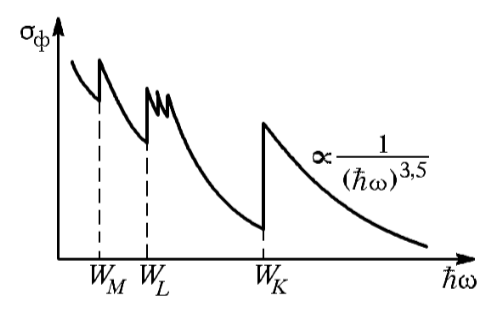
\includegraphics[scale = 0.8]{p1.png}
    \caption{Зависимость сечения фотоэффекта от энергии $\gamma$-квантов}
    \label{p1}
    \end{center}
\end{figure}

Вероятность фотоэффекта быстро возрастает при переходе от легких к тяжелым элементам и резко падает
с увеличением энергии гамма-квантов. При возрастании энергии сечение скачкообразно возрастает, когда 
становится возможным выбивание электронов с очередной оболочки. Фотоэффект является доминирующим механизмом
поглощения гамма-квантов при не очень высоких энергиях.



\subsection{Комптоновское рассеяние}

Комптон эффект - упругое столкговение гамма-кванта с электроном. Этот эффект происходит на свободных 
или слабосвязанных электронах в отличие от фотоэффекта. Роль эффекта Комптона становиться существенной 
только когда энергия гамма-квантов становится много больше энергии связи электронов в атоме. Атомные электроны
можно считать практиески свободными. \par 

Вертоятность Комптон эффекта сложно зависит от энергии гамма-квантов. В случае, когда энергия 
гамма-кванта много больше энергии покоя электрона:

\begin{equation}
    \sigma_k = \pi r^2 \frac{mc^2}{\hbar \omega} \left ( \ln{\frac{2 \hbar \omega}{mc^2}}+ \frac{1}{2} \right )
\end{equation}

$r \approx 2.8 \cdot 10^{-13} \; см$ - классический радиус электрона. Следует, что сечение комптон-эффекта 
с ростом энергии фотонов падает не так резко, как сечение фотоэффекта. \par 

Сечение $\sigma_k$ относится к одному свободному электрону, а сечение фотоэффекта рассчитано на атом. 
Значит комптоновское рассеяние становится в $Z$ раз больше. \par 

Комптоновский коэффициент линейного ослабления $\mu_k$ связан с сечением $\sigma_k$ через плотность слабосвязанных 
электронов $n$:

\begin{equation}
    \mu_k = \sigma_k \cdot n
\end{equation}

Отметим, что эффект Комптона приводит не к поглащению, а к рассеянию гамма-кватнов. 



\subsection{Генерация электрон-позитронных пар}

При энергиях $\gamma$-лучей, превышающих $2mc^2 = 1.02 \; МэВ$, становится возможен процесс образования 
электрон-позитронных пар. Рождение пар происходит в эл. поле ядер, вероятность процесса $\sim \; Z^2$ и сложным
образом зависит от энергии фотона. \par 

При энергиях более 1.02 МэВ фотоэффект почти не играет роли даже для самых тяжелых ядер. Вероятность образования пар 
сравнительна с вероятностью комптоновского рассеяние. Рождение пар существенно только для самых тяжелых элементов. 
Для свинца вероятность рождения пар сравнивается с вероятностью комптоновского эффекта только при 4.7 МэВ.



\subsection{Полный коэффициент ослабления}

Полный линейный кожффициент $\mu$ равен сумме коэффициентов для всех трех рассмотренных процессов.
На рис. \ref{p2}

\begin{figure}[H]
    \begin{center}
    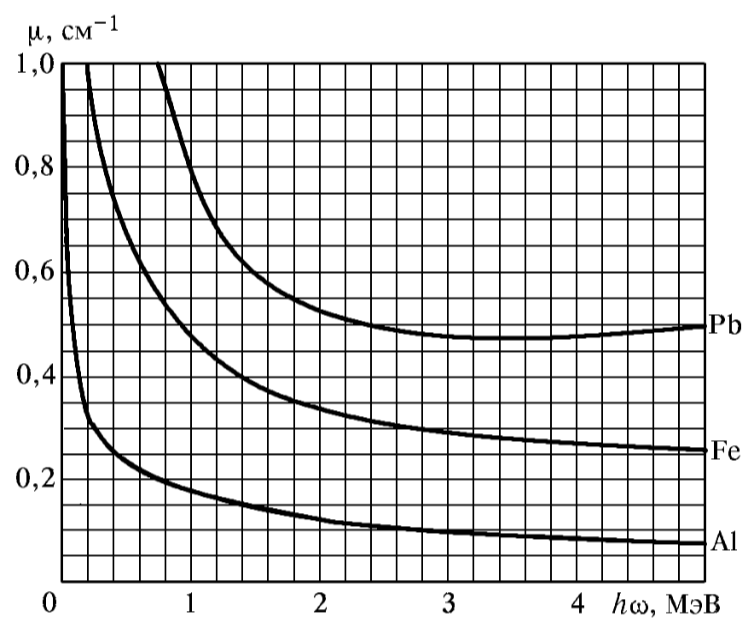
\includegraphics[scale = 0.8]{p2.png}
    \caption{Полные коэффициенты ослабления потока $\gamma$ - лучей в алюминии, железе и свинце}
    \label{p2}
    \end{center}
\end{figure}

\begin{figure}[H]
    \begin{center}
    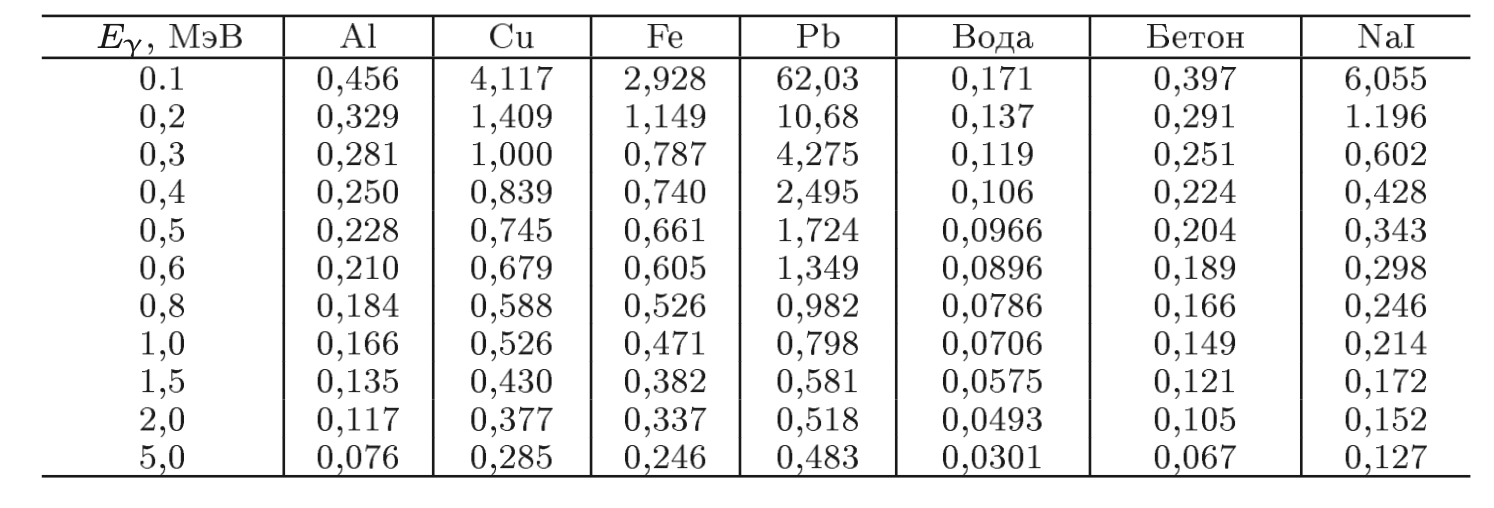
\includegraphics[scale = 0.6]{p3.png}
    \caption{Полные коэффициенты ослабления потока $\gamma$ - лучей в разных веществах}
    \label{p3}
    \end{center}
\end{figure}

Получим формулу (1). Рассмотрим опыты в хорошей геометрии, когда $\gamma$ - кванты выводит из пучка фотоэлектрическое поглощение, комптоновское
рассеяние и генерация пар. \par 

При прохождении через вещество меняется количество, а не энергия квантов в пучке, значит коэффициент 
$\mu$ не зависит от длины пути. Пусть $-dN$ число гамма-квантов, выбывших из пучка на пути $dl$, это число 
пропорционально имеющемуся их числу $N$ и пройденному пути $dl$:

\begin{equation}
    -dN = \mu N dl
\end{equation}

Интегрируем от нулевой толщины до заданной:

\begin{equation}
    N = N_0 e^{-\mu l}
\end{equation}

Получили ф-лу (1).\par 

В плохой геометрии, когда рассеянные под небольшими углами кванты остаются в пучке эта формула не применима, однако,
хорошо работает :). \par
Причина хорошего согласия в том, что гамма-кванты с энергие 1-2 МэВ, потерявшие энергию из-за комптоновского ослабления, 
быстро выбывают из пучка аз-за резкого увеличения сечений $\sigma_ф$ и $\sigma_k$. В данной работе коэффициент ослабления $\mu$
измеряектся в хорошей геометрии:

\begin{equation}
    \mu - \frac{1}{l} \ln{\frac{N_0}{N}}
\end{equation}



\section{Экспериметнальная установка}

Схема установки показана на рис. \ref{setup1}
Свинцовый коллиматор выделяет узкий параллельный пучок гамма-квантов, проходящий через набор поглотителей П.
Сигналы от счетсчика усиливаются и регистрируются пересчетным приьором ПП. \par 

При недостаточно хорошей геометрии в результате опытов могут быть погрешности. В реальности всегда имеется 
вероятность, что гамма-квант провзаимодействует в поглатителе несколько раз до того, как попадет в детектор (рис. \ref{setup2})
Чтобы этого избежать сцинтилляционный счетсчик расположен на больом расстоянии от источника гамма-квантов, а полглотители 
имеют небольшие размеры, также поглотители следует размещать на небольшом расстоянии друг от друга. 

\begin{figure}[H]
    \begin{center}
    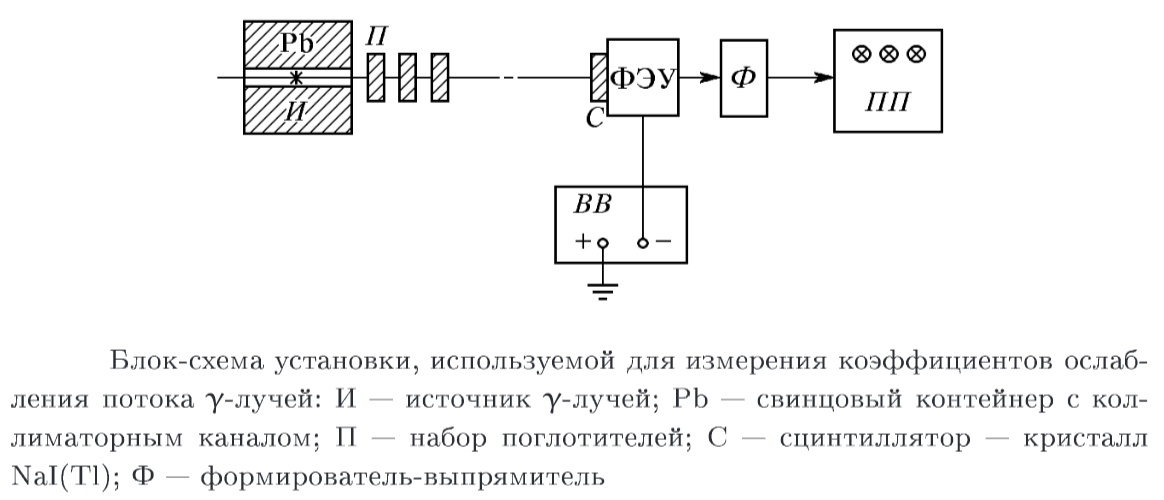
\includegraphics[scale = 0.8]{setup1.png}
    \caption{}
    \label{setup1}
    \end{center}
\end{figure}

\begin{figure}[H]
    \begin{center}
    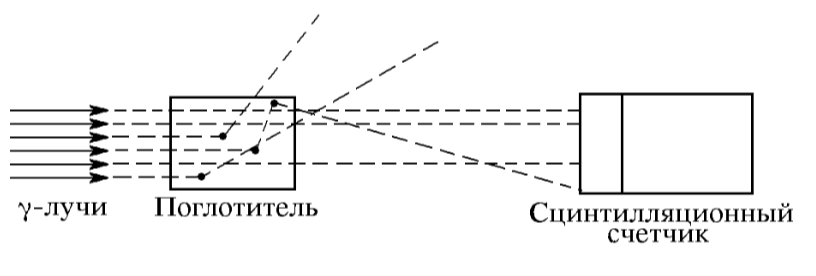
\includegraphics[scale = 0.8]{setup2.png}
    \caption{Схема рассеяния гамма-квантов в поглотителе}
    \label{setup2}
    \end{center}
\end{figure}



\section{Ход работы}

\begin{enumerate}
    \item  Включим пересчетный прибор и высоковольтный выпрямитель. Прогреем их.
    

    \item Измерим скорость счета с свинцовой пробкой и без, она резко увеличилась как только убрали свинцовую пробку.
    Данные занесем в таблицу на рис.\ref{t4}

    \begin{figure}[H]
        \begin{center}
        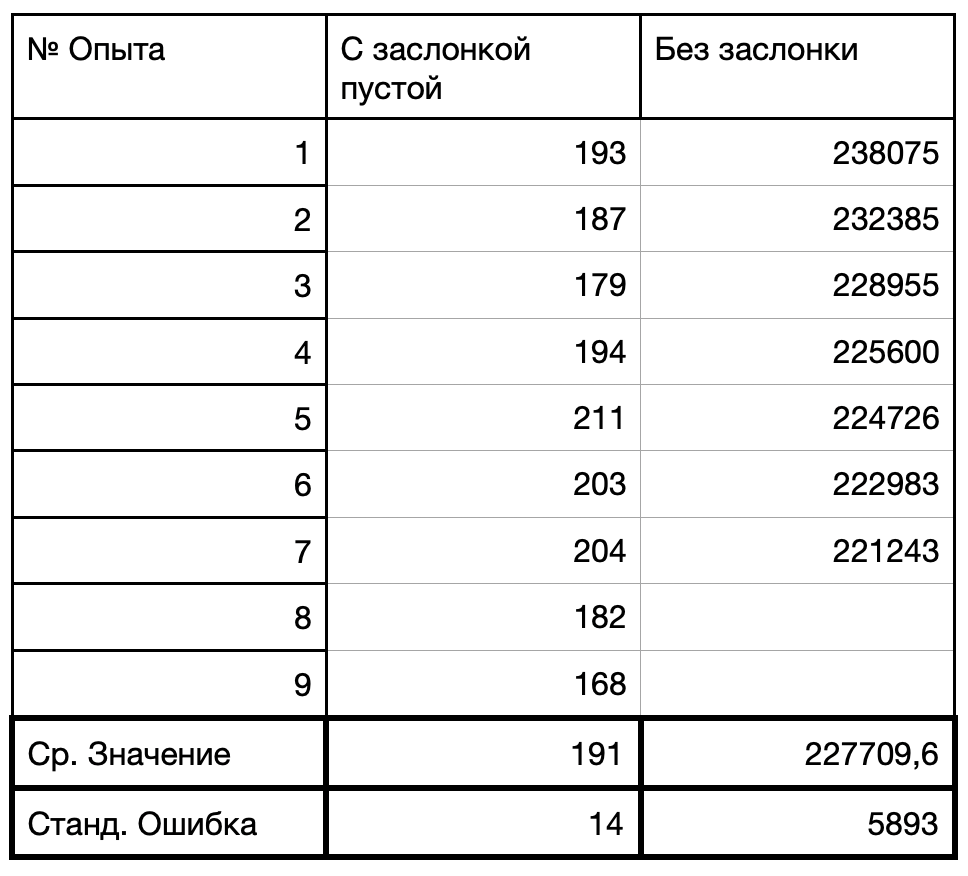
\includegraphics[scale = 0.42]{t4.png}
        \caption{Измернеие с и без свинцовой пробки}
        \label{t4}
        \end{center}
    \end{figure}


    \item Исследуем поглощение гамма-лучей в свинце, железе и алюминии, данные занесем в таблицы
    на рис. \ref{t1}, \ref{t3}, \ref{t2}

    \begin{figure}[H]
        \begin{center}
        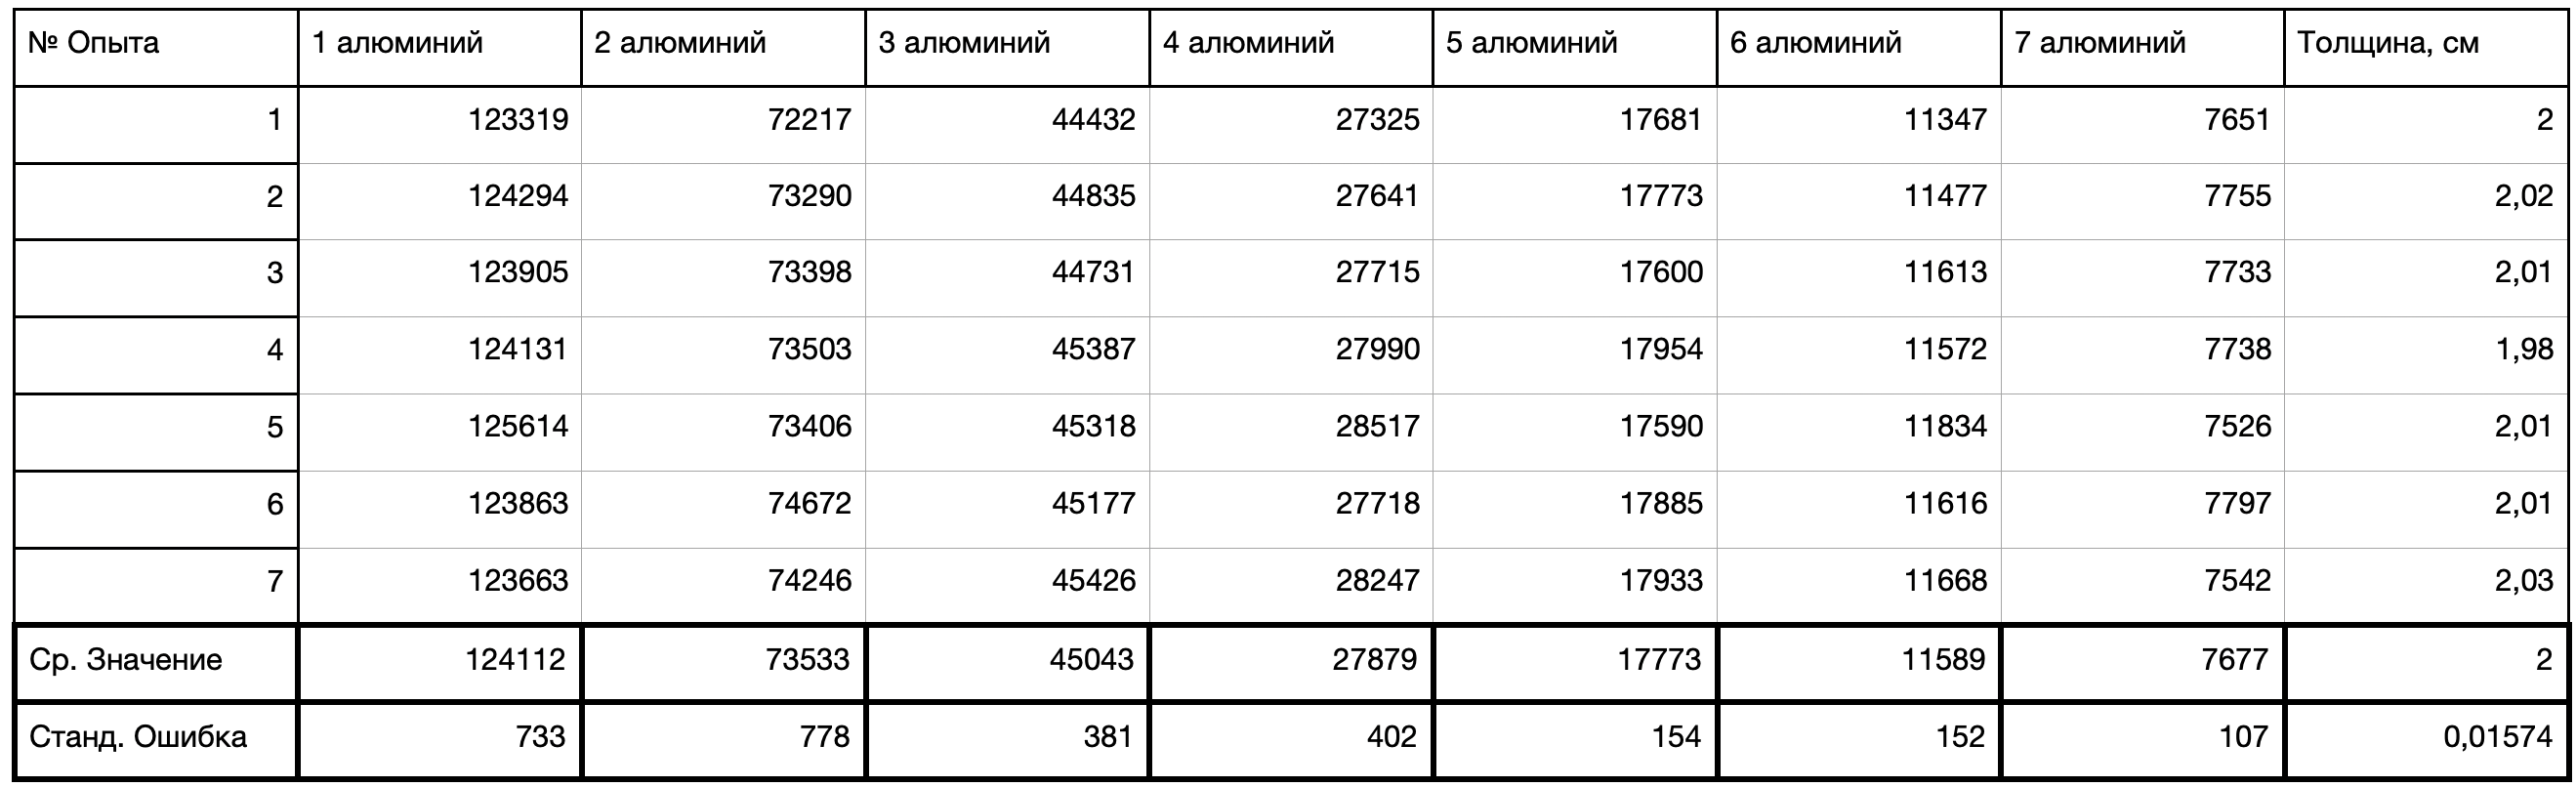
\includegraphics[scale = 0.4]{t1.png}
        \caption{Алюминий}
        \label{t1}
        \end{center}
    \end{figure}

    \begin{figure}[H]
        \begin{center}
        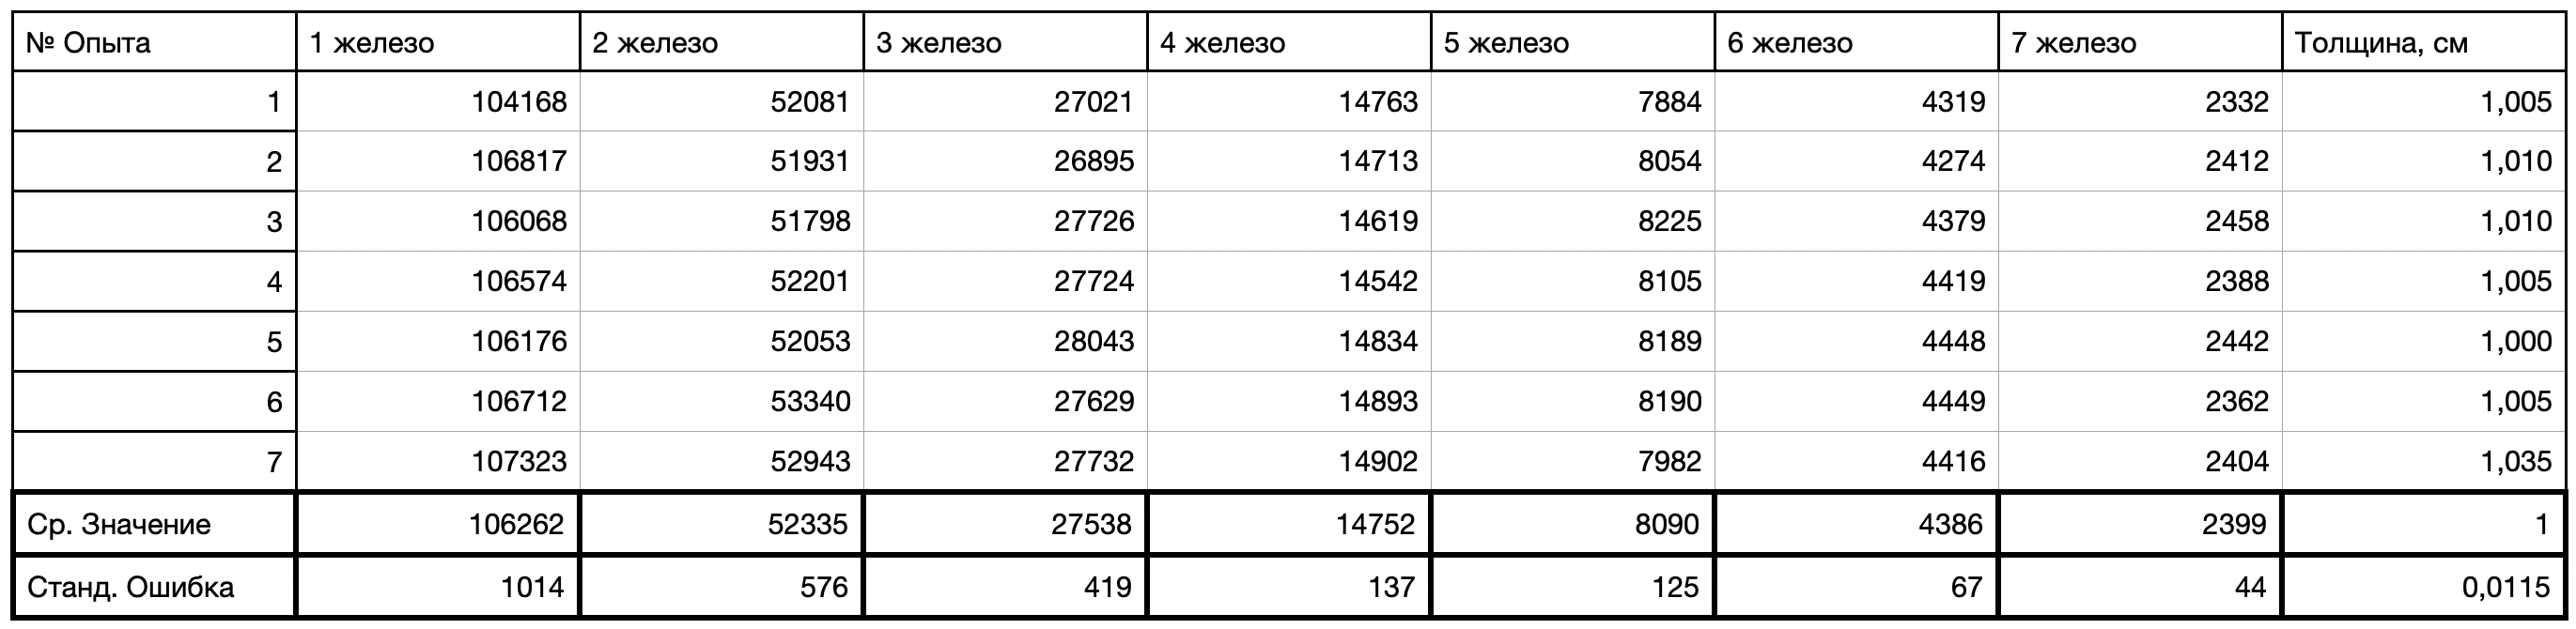
\includegraphics[scale = 0.4]{t3.png}
        \caption{Железо}
        \label{t3}
        \end{center}
    \end{figure}

    \begin{figure}[H]
        \begin{center}
        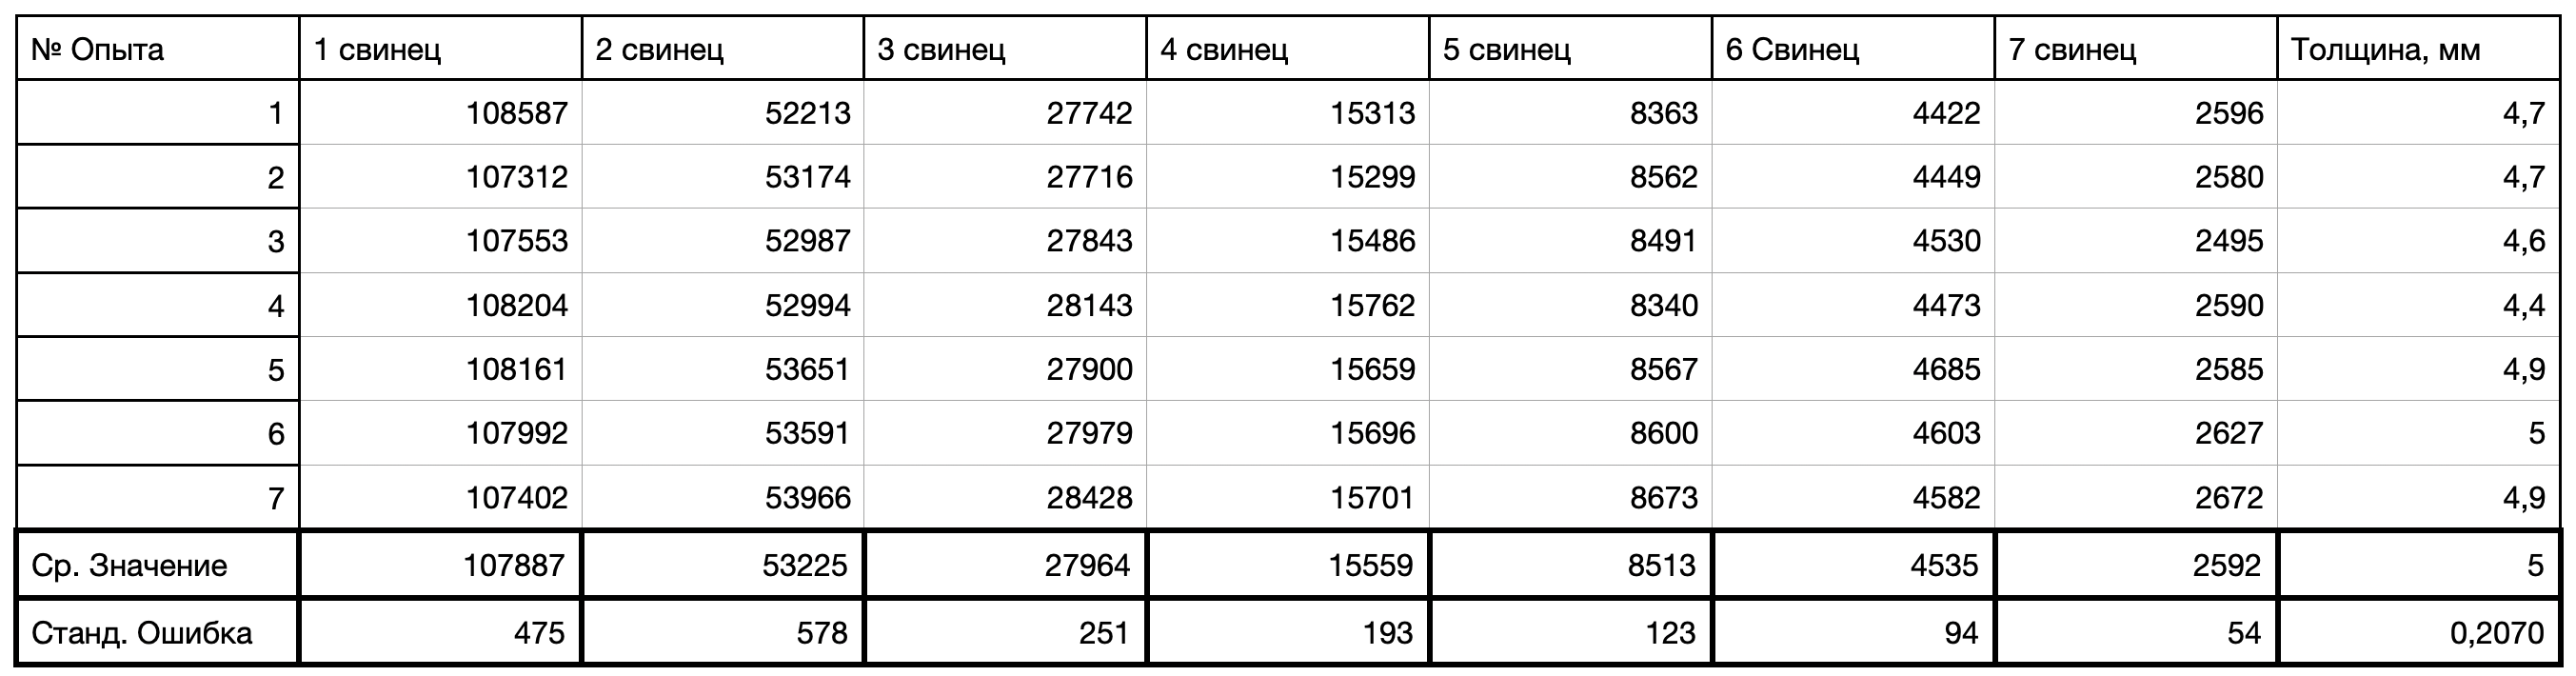
\includegraphics[scale = 0.4]{t2.png}
        \caption{Свинец}
        \label{t2}
        \end{center}
    \end{figure}


    \item Для каждого вида поглотителей построим зависимость $\ln{N}(l) = \ln{N_0} -  l\cdot \mu $
    на рис. \ref{Al}, \ref{Pb}, \ref{Fe}:

    Откуда получим линейный коэффициент $\mu$ как тангенс угла наклона:

    $$\mu_{Al} = 0.237 \pm 0.004 (\pm 1.7 \%) \; [см^{-1}]$$
    $$\mu_{Pb} = 1.272 \pm 0.020 (\pm 1.6 \%) \; [см^{-1}]$$
    $$\mu_{Fe} = 0.634 \pm 0.008 (\pm 1.3 \%) \; [см^{-1}]$$

    По линейным коэффициентам рассчитаем коэффициенты $\mu'$ по ф-ле (1) следует, что:
    $\mu' = \frac{\mu \cdot l}{m_1}$
    
    $$\mu'_{Al} = 0.087 \pm 0.002 (\pm 1.9 \%) \; [см^{2}/г]$$
    $$\mu'_{Pb} = 0.112 \pm 0.005 (\pm 4.4 \%) \; [см^{2}/г]$$
    $$\mu'_{Fe} = 0.081 \pm 0.001 (\pm 4.3 \%) \; [см^{2}/г]$$

    \begin{figure}[H]
        \begin{center}
        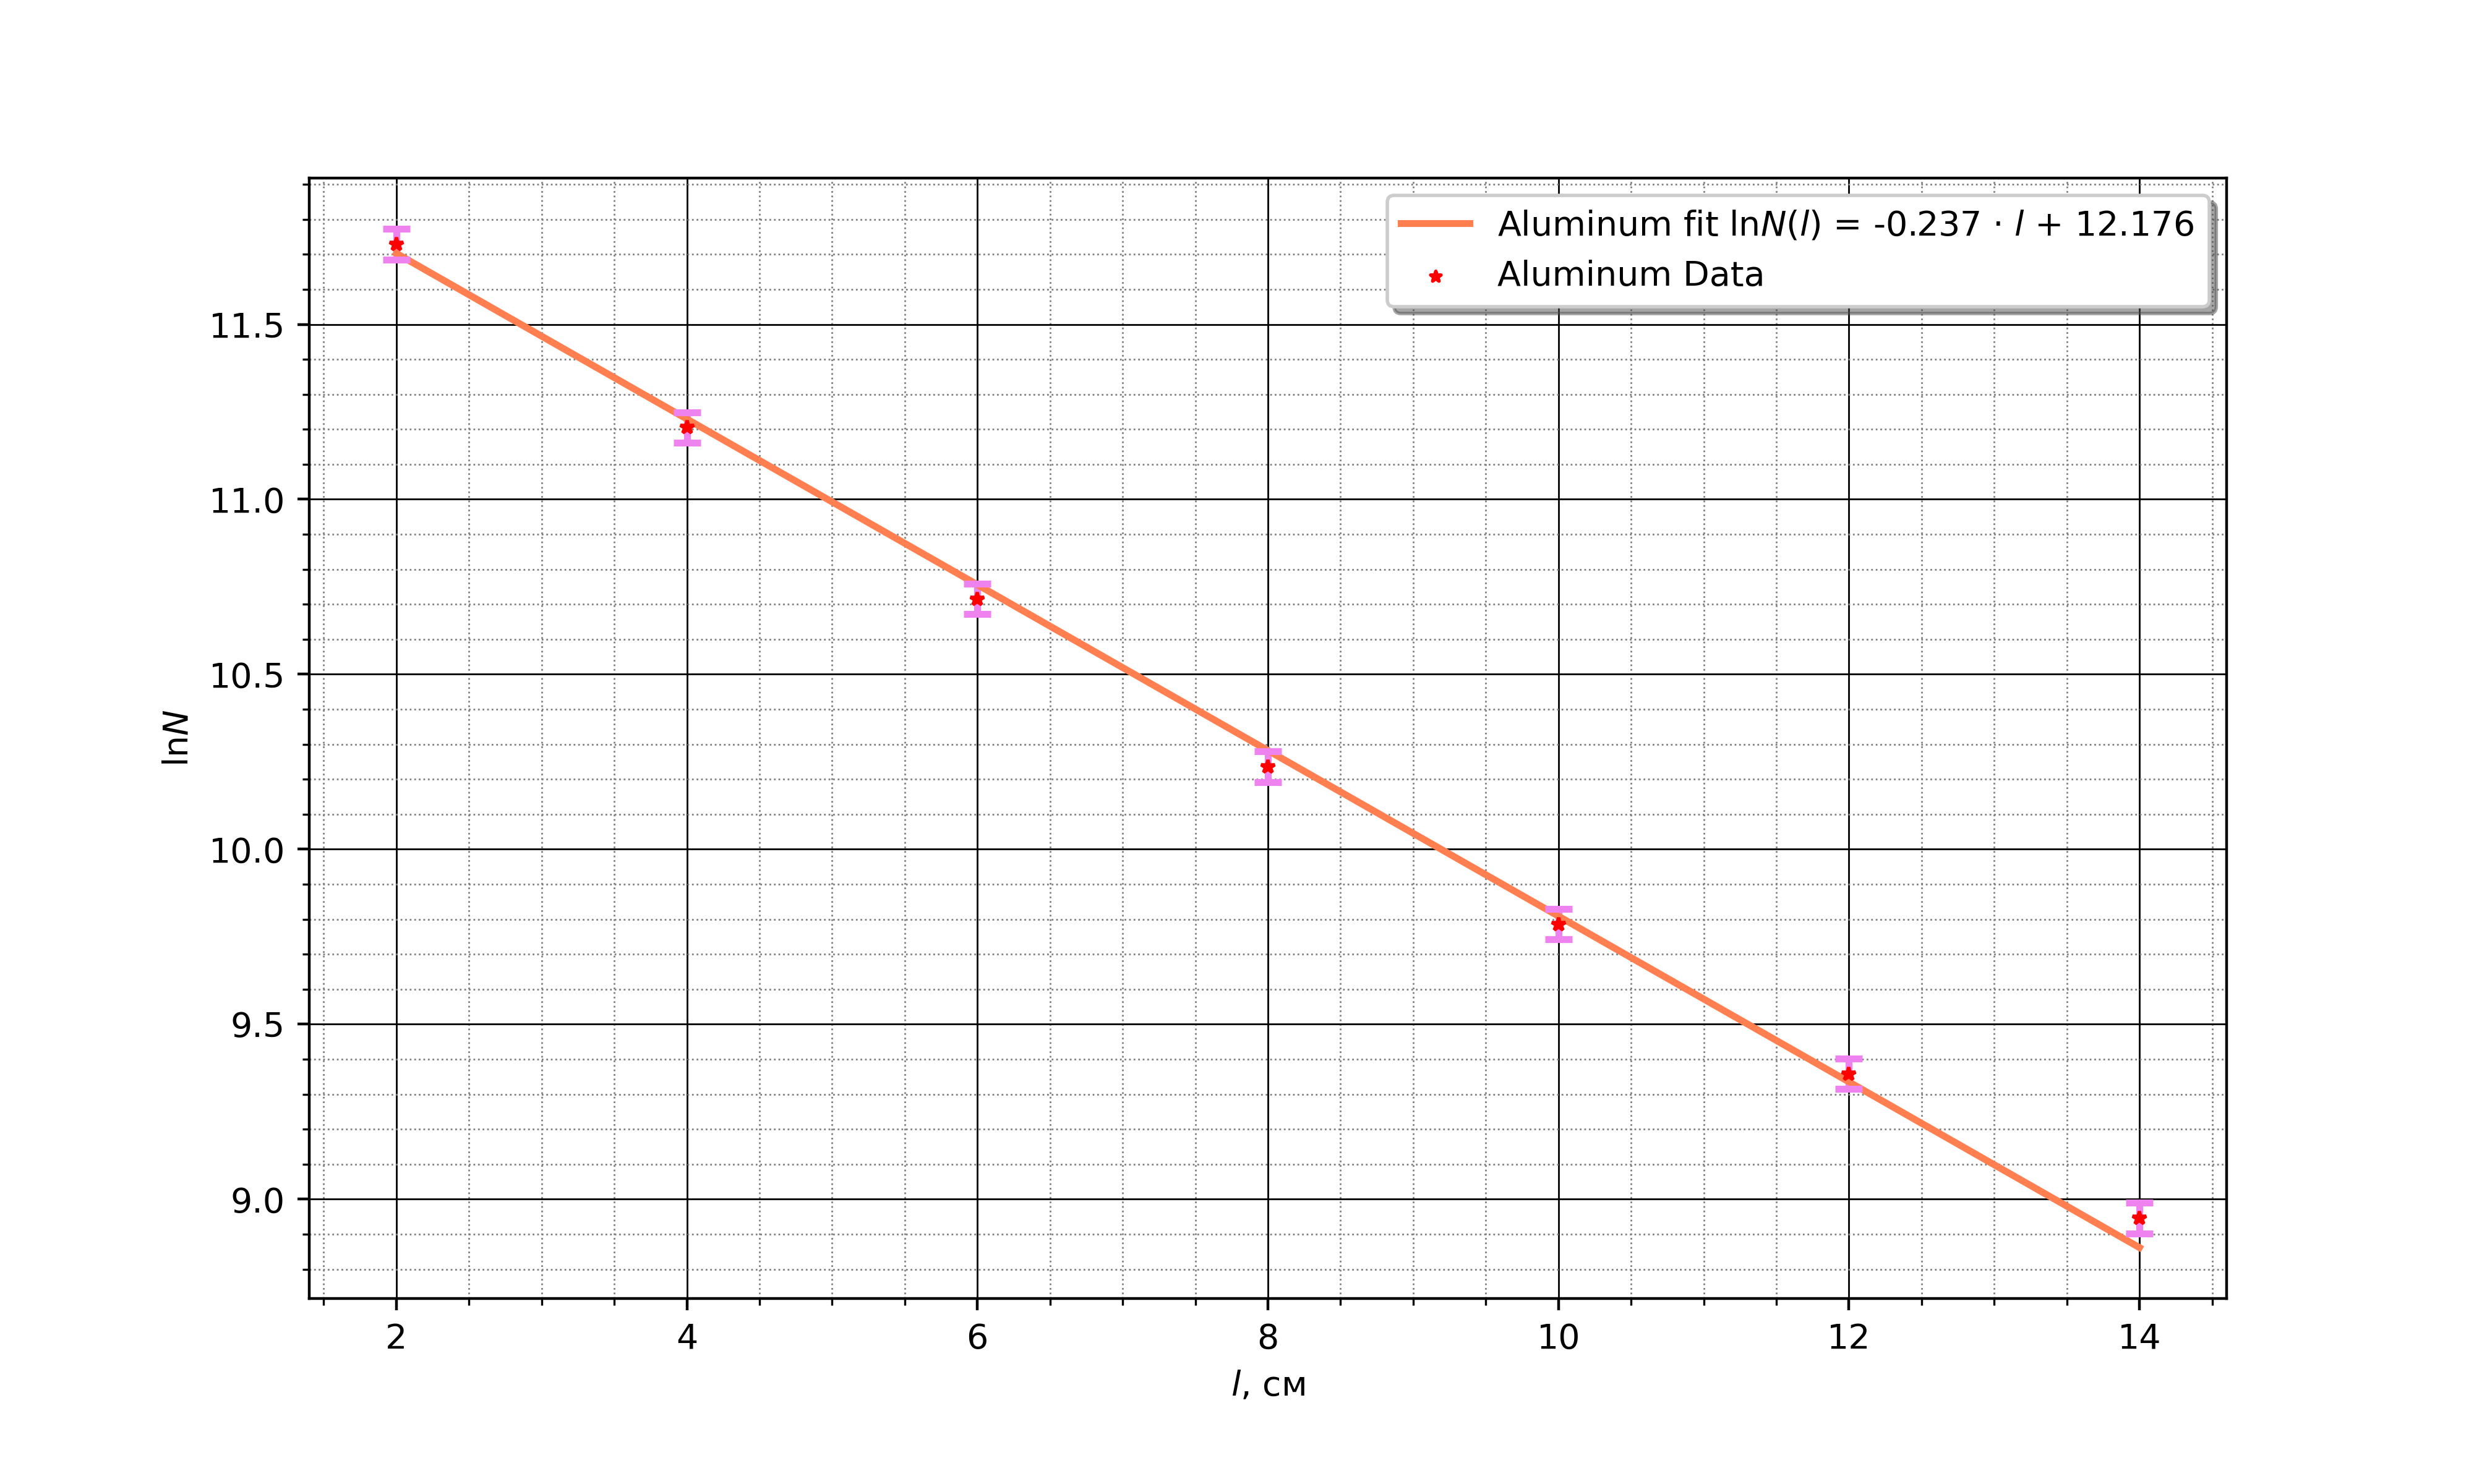
\includegraphics[scale = 0.65]{Al.png}
        \caption{Зависимость $\ln{N}(l) = \ln{N_0} -  l\cdot \mu $ для алюминия}
        \label{Al}
        \end{center}
    \end{figure}

    \begin{figure}[H]
        \begin{center}
        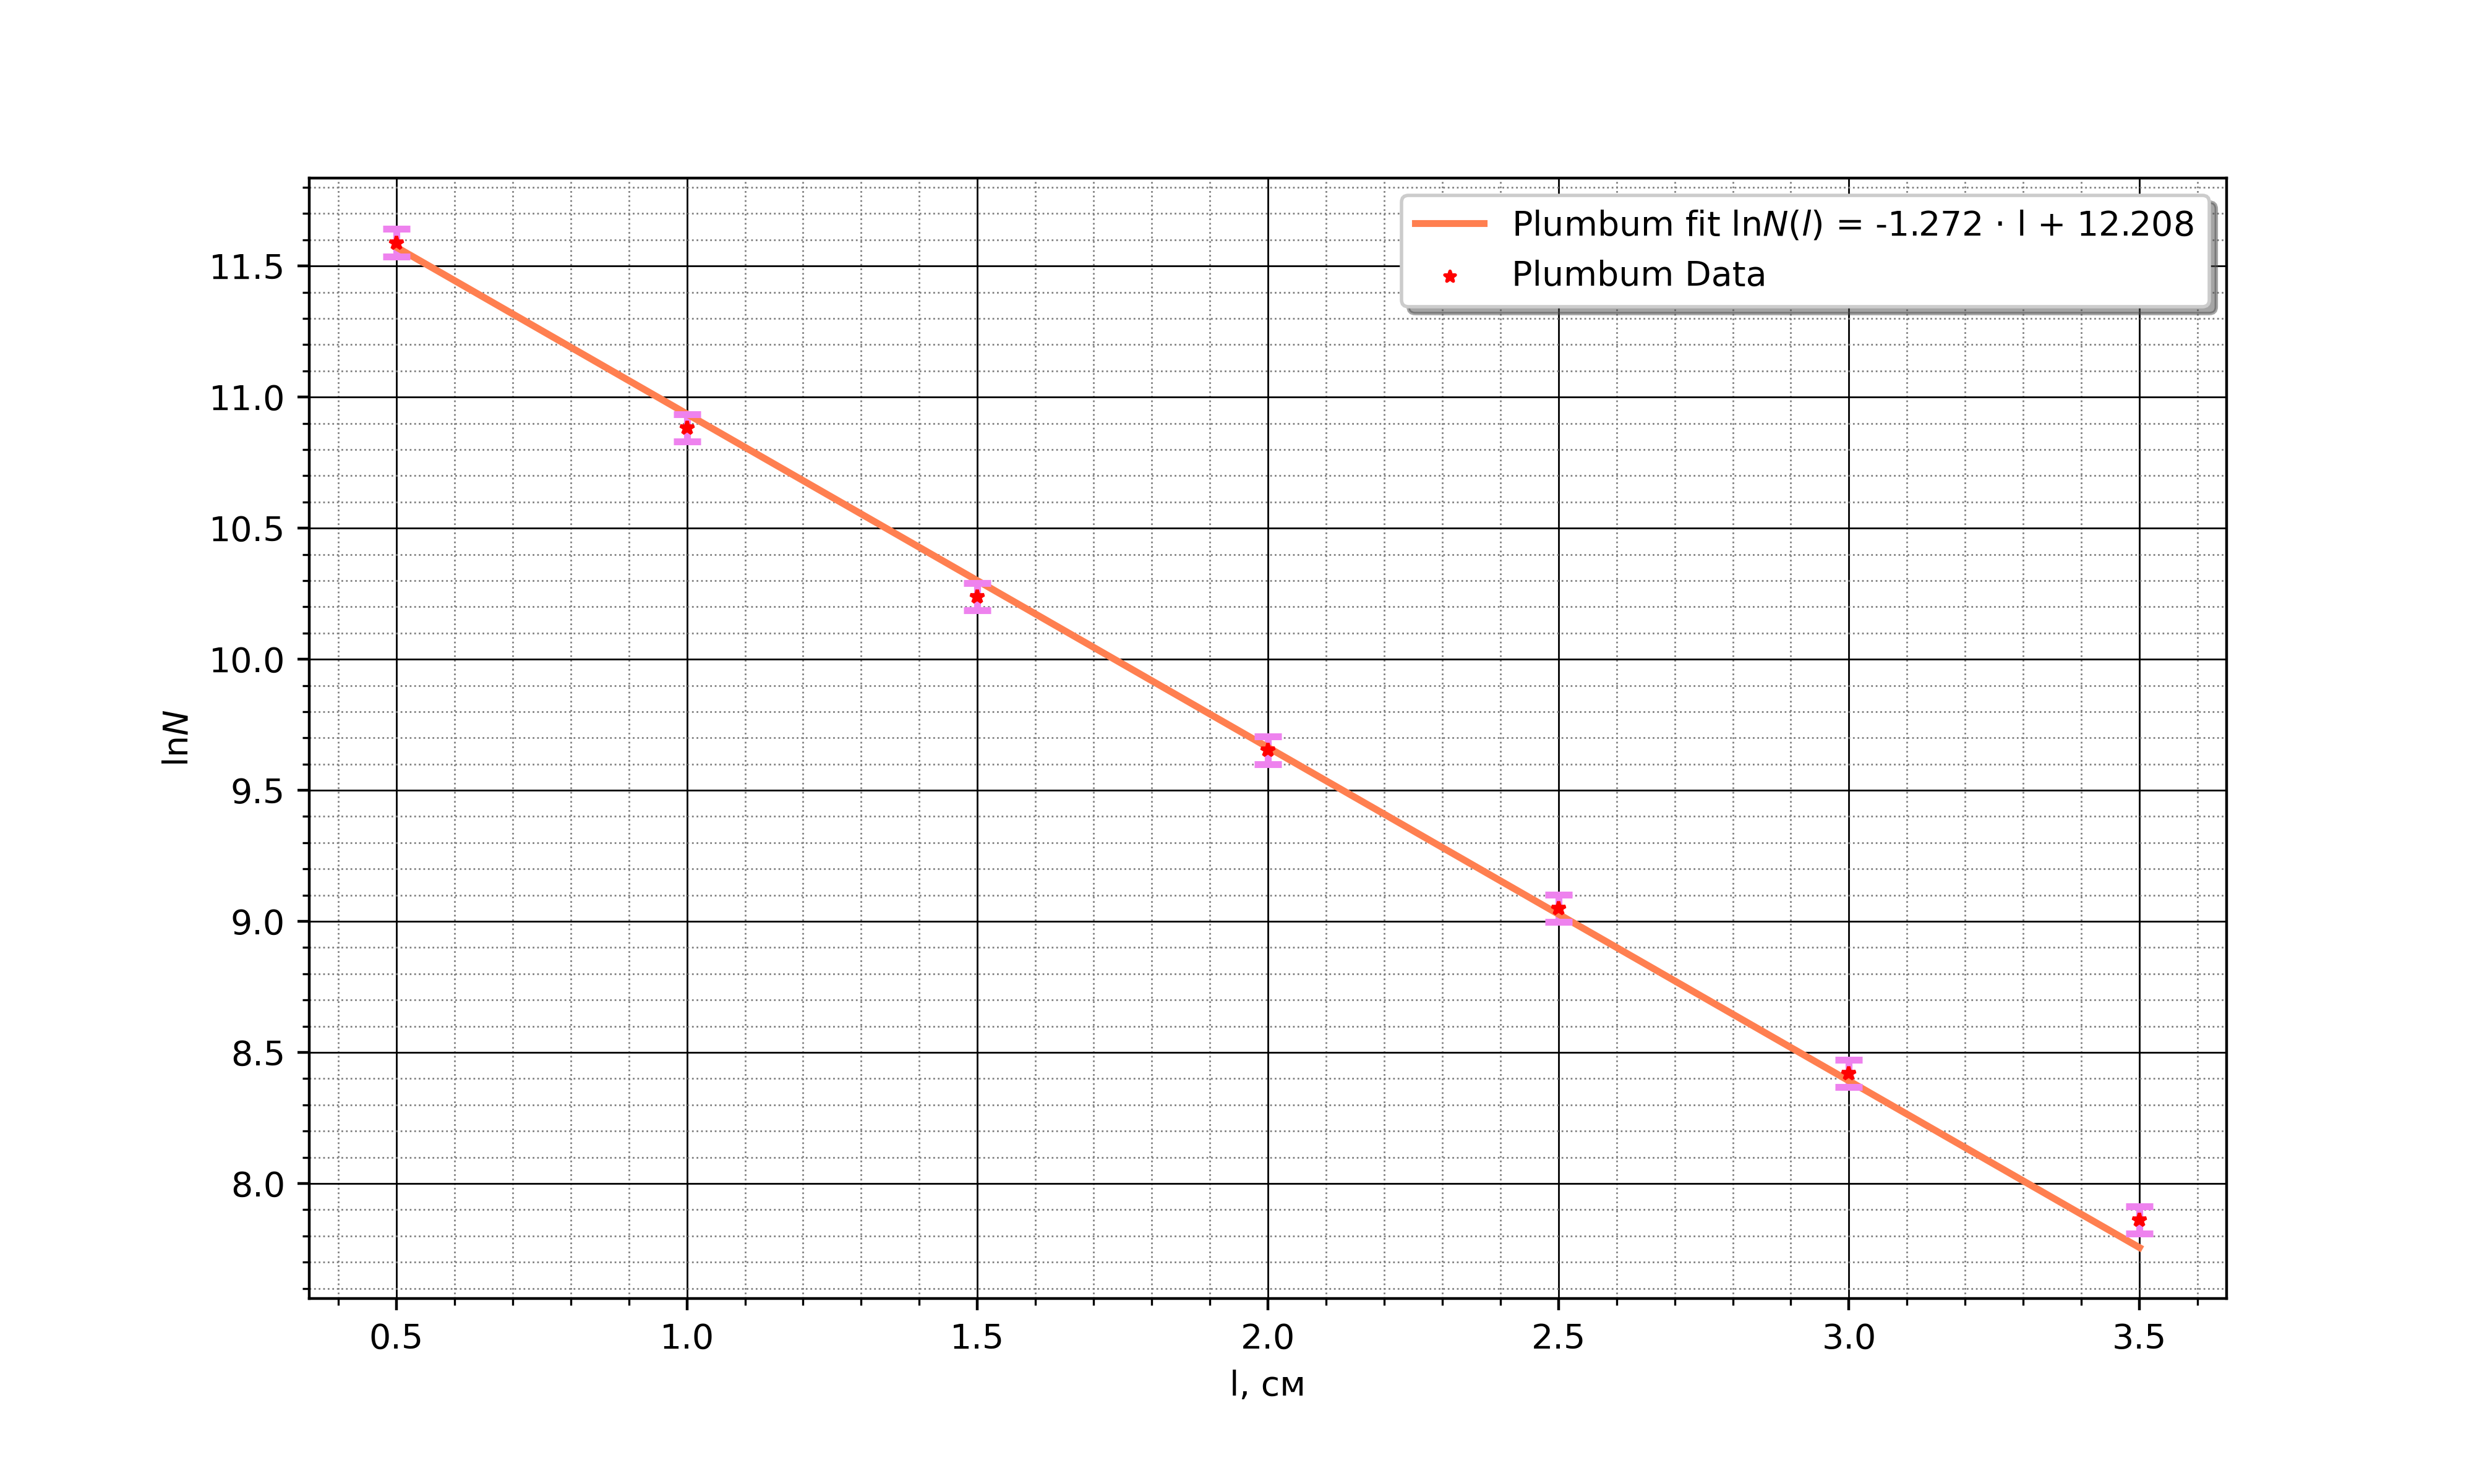
\includegraphics[scale = 0.65]{Pb.png}
        \caption{Зависимость $\ln{N}(l) = \ln{N_0} -  l\cdot \mu $ для свинца}
        \label{Pb}
        \end{center}
    \end{figure}

    \begin{figure}[H]
        \begin{center}
        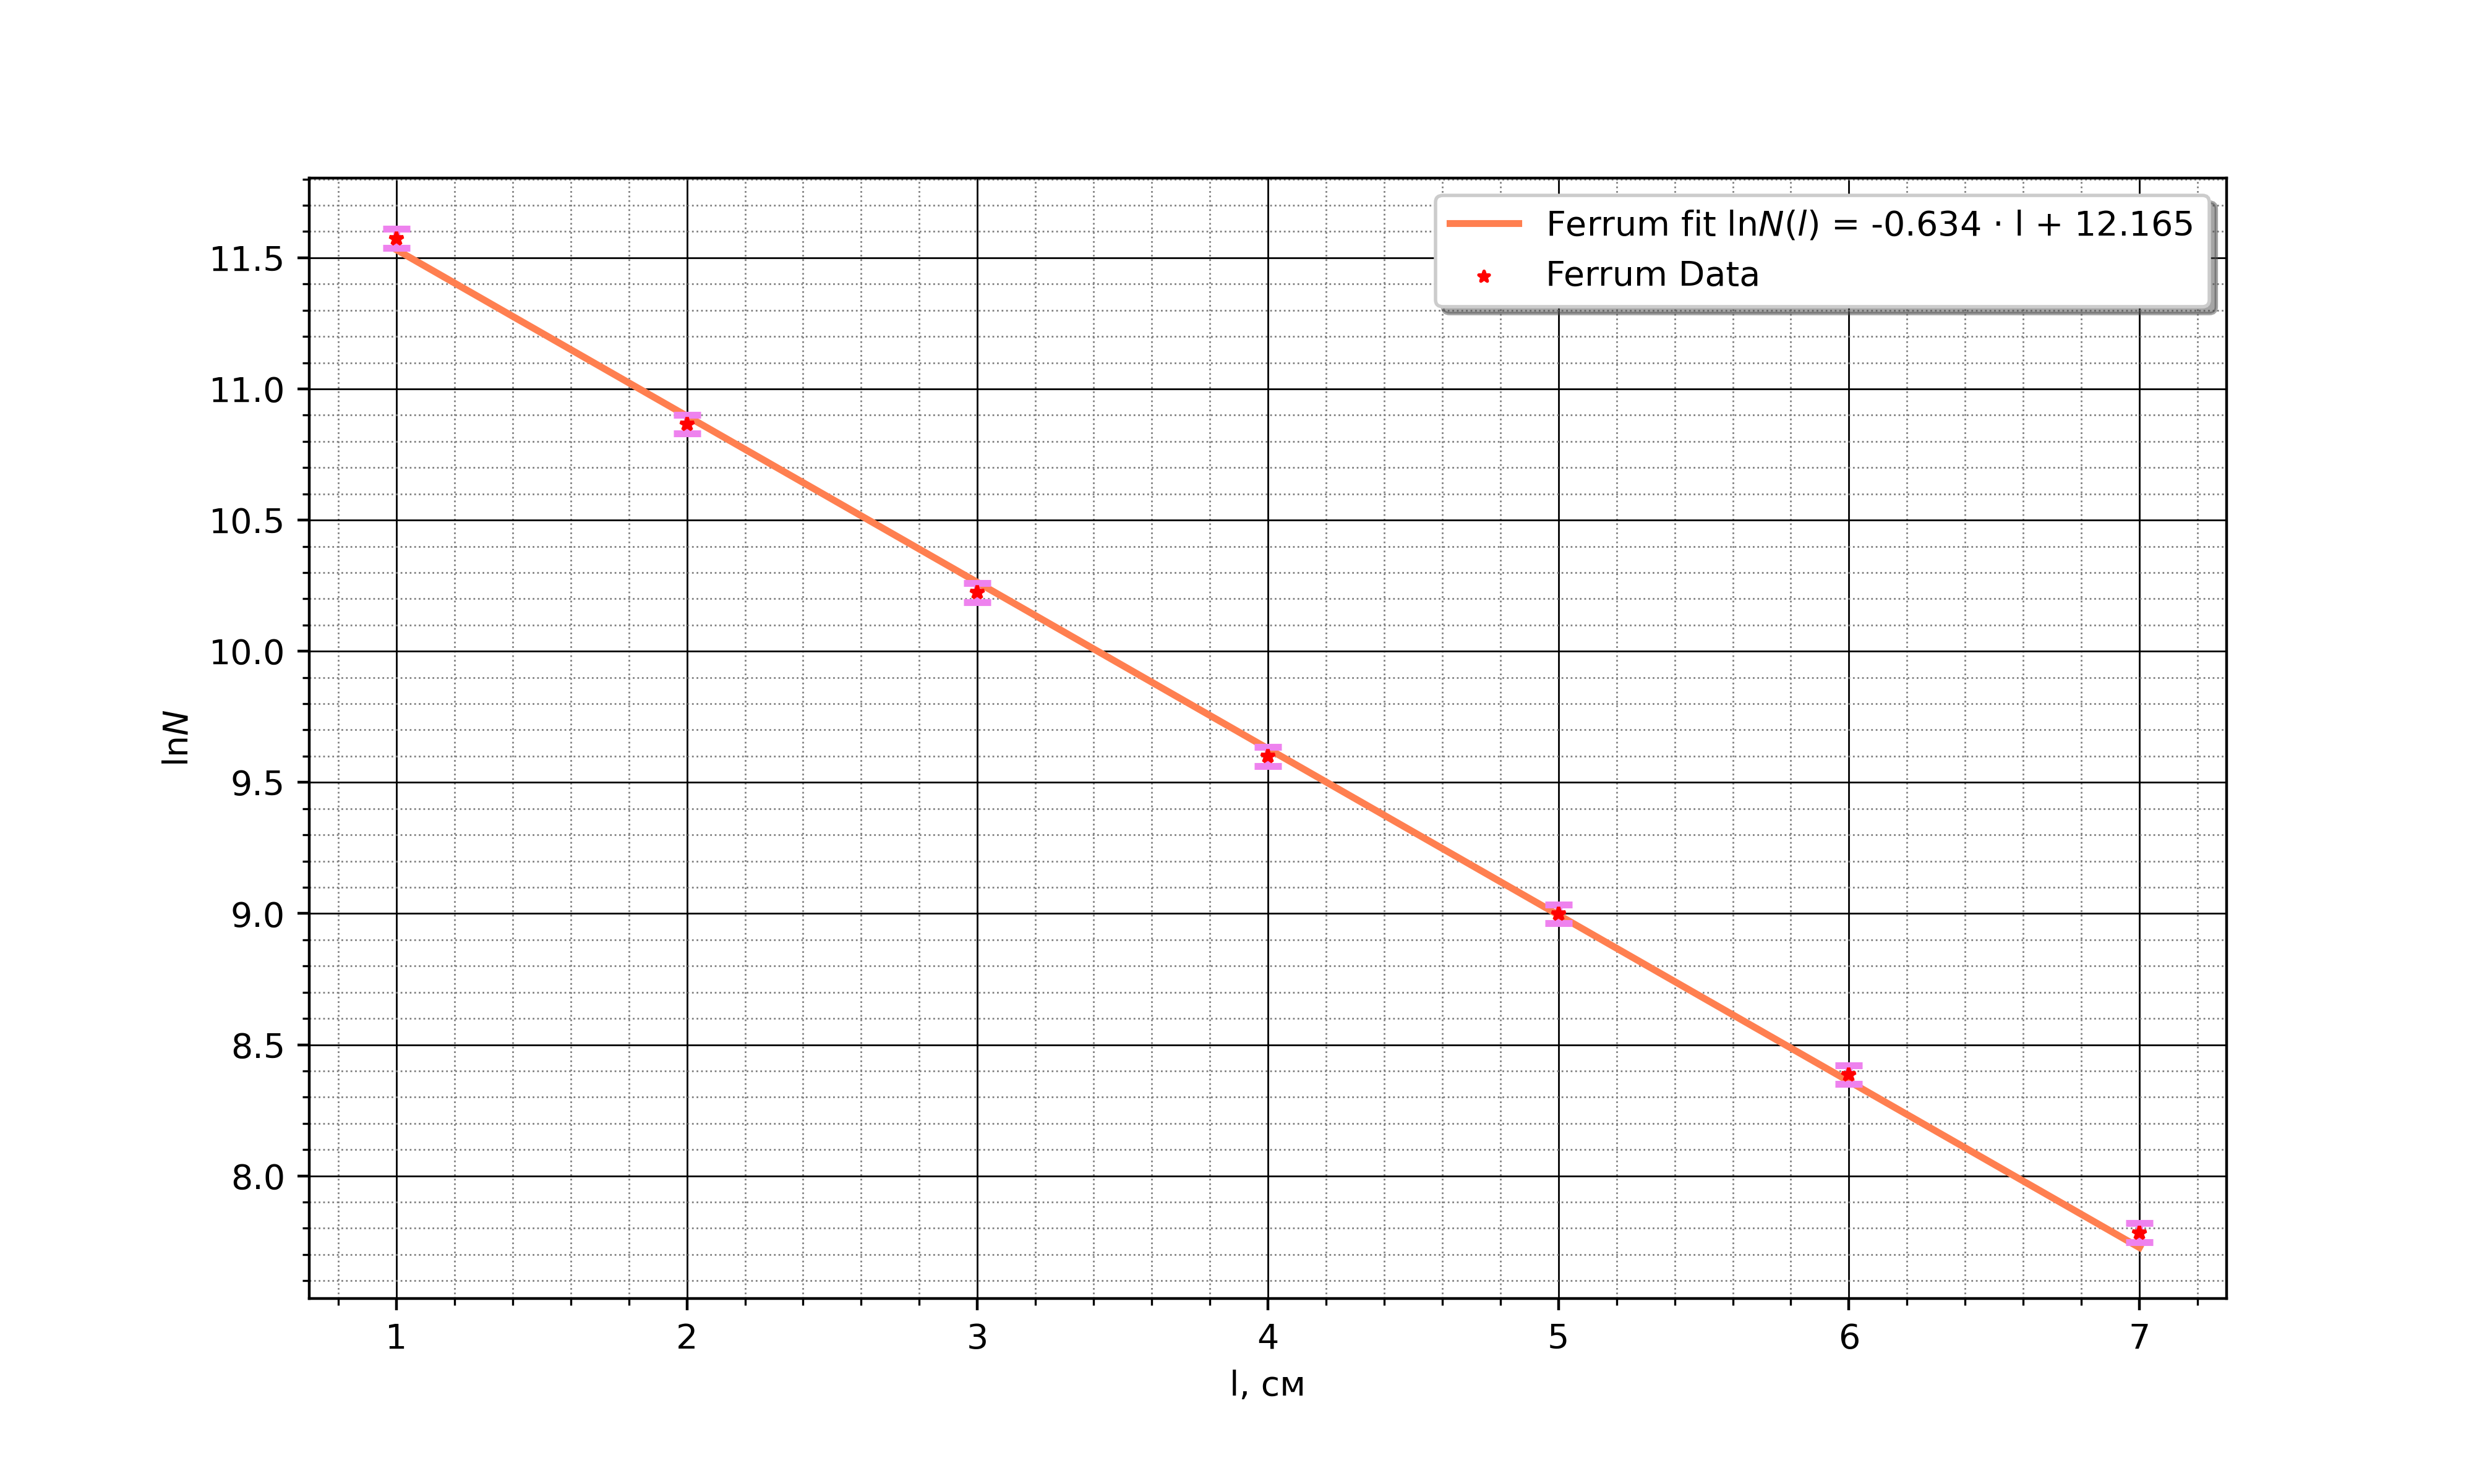
\includegraphics[scale = 0.65]{Fe.png}
        \caption{Зависимость $\ln{N}(l) = \ln{N_0} -  l\cdot \mu $ для железа}
        \label{Fe}
        \end{center}
    \end{figure}


    \item Определим среднюю энерегию гамма-квантов по графику с рис. \ref{p2} и таблице с рис. \ref{p3}. 

    $$\overline{E_{\gamma}} \approx 0.55 \pm 0.06 (\pm 10.5 \%)\; [МэВ]$$
\end{enumerate}



\section{Вывод}

В данной работе мы с помощью сцинтилляционного счетсчика измерили линейные коэффициенты ослабления потока $\gamma$ - лучей в свинце,
железе и алюмини; определили среднюю энергию гамма-лучей, излучаемых источником.




\end{document}